%!TEX root = ../Main.tex

\chapter{Exercise 4}

This exercise will deal with the steps to implement a matrix multiplier. 

At first three global variables of the data structure \textbf{vectorArray} called \textbf{pInst}, \textbf{aInst} and \textbf{bTInst} were created. 

Next a function called \textbf{setInputMatrices()} was implemented. This function will initialize two matrices. Below is a code snippet of the implementation. The comments in the code explains how the each element in the matrices are initialized. 

 \begin{lstlisting}
 void setInputMatrices()
 {
 //Set matrix a
 // A, row 0
 aInst[0].comp[0] = 1;
 aInst[0].comp[1] = 2;
 aInst[0].comp[2] = 3;
 aInst[0].comp[3] = 4;
 
 // A, row 1
 aInst[1].comp[0] = 5;
 aInst[1].comp[1] = 6;
 aInst[1].comp[2] = 7;
 aInst[1].comp[3] = 8;
 
 // A, row 2
 aInst[2].comp[0] = 9;
 aInst[2].comp[1] = 10;
 aInst[2].comp[2] = 11;
 aInst[2].comp[3] = 12;
 
 // A, row 3
 aInst[3].comp[0] = 13;
 aInst[3].comp[1] = 14;
 aInst[3].comp[2] = 15;
 aInst[3].comp[3] = 16;
 
 //Set matrix bT
 // A, row 0
 bTInst[0].comp[0] = 1;
 bTInst[0].comp[1] = 2;
 bTInst[0].comp[2] = 3;
 bTInst[0].comp[3] = 4;
 
 //Set matrix bT
 // A, row 1
 bTInst[1].comp[0] = 1;
 bTInst[1].comp[1] = 2;
 bTInst[1].comp[2] = 3;
 bTInst[1].comp[3] = 4;
 
 //Set matrix bT
 // A, row 2
 bTInst[2].comp[0] = 1;
 bTInst[2].comp[1] = 2;
 bTInst[2].comp[2] = 3;
 bTInst[2].comp[3] = 4;
 
 //Set matrix bT
 // A, row 3
 bTInst[3].comp[0] = 1;
 bTInst[3].comp[1] = 2;
 bTInst[3].comp[2] = 3;
 bTInst[3].comp[3] = 4;
 }
 
 \end{lstlisting}
 
 Next a function called \textbf{displayMatrix(vectorArray matrix)} was implemented. 
 As the name of the function strongly implies, this function will display a given matrix in the  terminal. To implement \textbf{displayMatrix(vectorArray matrix)} a function called \textbf{displayMatrixRow(vectorArray matrix, int row)} is implemented in addition. That's because we have to display the matrix row for row.
 Below is a code snippet of the implemented function.
 
 \begin{lstlisting}
 void displayMatrix(vectorArray matrix)
 {
 xil_printf("[\r\n");
 displayMatrixRow(matrix,0);
 displayMatrixRow(matrix,1);
 displayMatrixRow(matrix,2);
 displayMatrixRow(matrix,3);
 xil_printf("]\r\n");
 }
 
 void displayMatrixRow(vectorArray matrix, int row)
 {
 xil_printf("%d %d %d %d \r\n", matrix[row].comp[0], matrix[row].comp[1], matrix[row].comp[2], matrix[row].comp[3]);
 }
 \end{lstlisting}
 
 Next a function called \textbf{multiMatrixSoft(vectorArray in1, vectorArray in2, vectorArray out)} was implemented, which is responsible for computing 4x4 matrix product of the expression \[ P = A x B^T \]
 
This function takes three input because its not possible to return a matrix. So the result matrix is given as the third input parameter, that way we can set the new value of the result matrix in the function. To iterate all combinations of the result matrix P to calculate the sum of products of each element in P, three nested for-loops were used. 
Below is a code snippet of the \textbf{multiMatrixSoft(vectorArray in1, vectorArray in2, vectorArray out)}

 \begin{lstlisting}
void multiMatrixSoft(vectorArray in1, vectorArray in2, vectorArray out)
{
	for (int row = 0 ; row < MSIZE; row++)
	{
		for (int col = 0 ; col < MSIZE; col++)
		{
			xil_printf("[%d,%d]\r\n", row, col);
			for (int i = 0 ; i < MSIZE ; i++)
			{
				out[row].comp[col] += in1[row].comp[i] * in2[row].comp[i];
			}
		}
	}
};
\end{lstlisting}

Next, we wanted to test the multiMatrixSoft function, and test the execution time in clock ticks. For this we implemented a timer, and two integers: \textbf{time\_SW\_pre} and \textbf{time\_SW\_post}. We use the \textbf{XScuTimer\_GetCounterValue(TimerInstancePtr)} to get the elapsed time before and after the execution and store it in the variables \textbf{time\_SW\_pre} and \textbf{time\_SW\_post}. We then subtract \textbf{time\_SW\_post} form \textbf{time\_SW\_pre} to get the excution time in clock ticks. Below is the a code snippet of this with comments. 


 \begin{lstlisting}
 XScuTimer Timer; /* Cortex A9 SCU Private Timer Instance */
 
 // PS Timer related definitions
 XScuTimer_Config *ConfigPtr;
 XScuTimer *TimerInstancePtr = &Timer;
 
// Multiply matrices in SW.
xil_printf("Calculating P in SW\r\n");
int time_SW_pre, time_SW_post;
XScuTimer_Start(TimerInstancePtr); 	// Start the timer
time_SW_pre = XScuTimer_GetCounterValue(TimerInstancePtr); // Get elapsed time
multiMatrixSoft(aInst, bTInst,pInst);
time_SW_post = XScuTimer_GetCounterValue(TimerInstancePtr); // Get elapsed time
int time_elapsed_SW = time_SW_pre-time_SW_post; // Calculate elapsed time
xil_printf("P = \r\n");
displayMatrix(pInst);

xil_printf("SW: %d\r\n",timeElapsed_SW); //print execution time
\end{lstlisting}

On \cref{fig:multiMatrixSoft} a screenshot of the terminal is displayed. It shows the two matrices that is being multiplied, their product and at the bottom the time it took to execute in clock cycles.  

\begin{figure}[H]
	\centering
	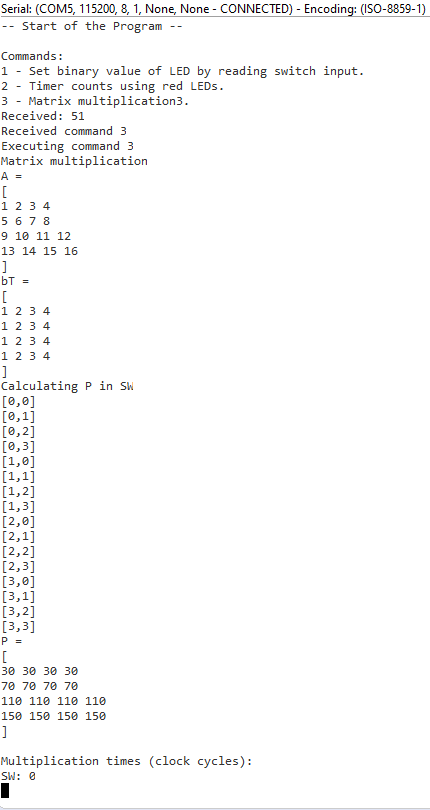
\includegraphics[width=0.8\textwidth]{Images/multiMatrixSoft.png}
	\caption{multiMatrixSoft result in terminal}
	\label{fig:multiMatrixSoft}
\end{figure}

 
 